\section[Planejamento em Intelig�ncia Artificial]{Planejamento em Intelig�ncia Artificial}

\begin{frame}
	
    \frametitle{Planejamento - Linha do Tempo}

	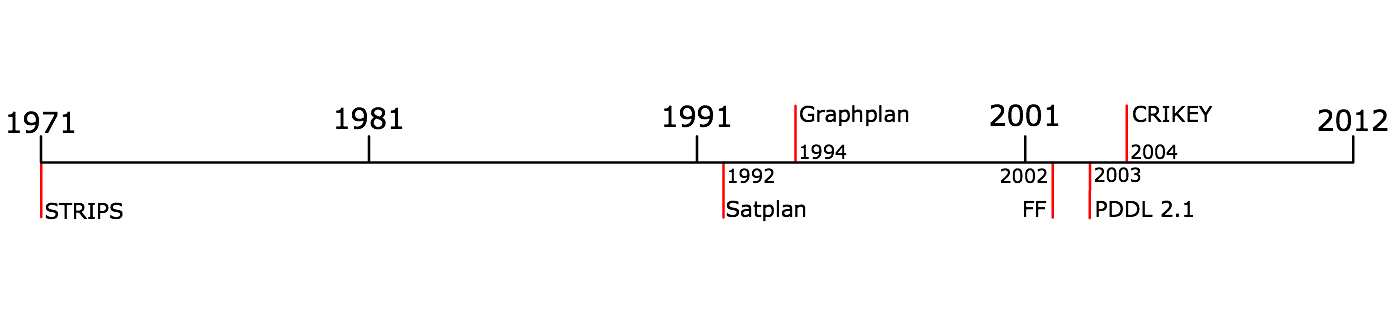
\includegraphics[width=\textwidth]{../images/fig_timeline.jpg}

    \begin{itemize}
		\item (1971) STRIPS (\emph{STranford Research Institute Problem Solver}) (RICHARD E.);
		\item (1992) \emph{Satplan} (A. HENRY);
		\item (1994) \emph{Graphplan} (L. AVRIM);
		\item (2002) FF (\emph{Fast-Forward}) (J. HOFFMANN);
		\item (2003) PDDL 2.1 \emph{Planning Domain Definition Language} (F. MARIA);
		\item (2004) \emph{CRIKEY} (H. KEITH);
    \end{itemize}
\end{frame}

\begin{frame}
    \frametitle{[Planejamento em Intelig�ncia Artificial}
    \begin{itemize}
		\item resolu��o de problemas do mundo real;
		\item planejamento:
		\begin{itemize}
			\item defini-se um estado inicial conhecido;
			\item defini-se um estado final desejado;
			\item busca-se por um conjunto de a��es que leve do inicial ao final;
		\end{itemize}
		\item problema de planejamento:
		\begin{itemize}
			\item encontrar uma sequ�ncia de a��es que, quando executada em um contexto que satisfa�a um estado inicial, vai atingir o objetivo;
		\end{itemize}
		\item plano:
		\begin{itemize}
			\item sequ�ncia de a��es que levam do estado inicial ao estado final;
		\end{itemize}
		\item PDDL:
		\begin{itemize}
			\item interface padr�o para utiliza��o de planejadores;
		\end{itemize}
		\item planejador CRIKEY:
		\begin{itemize}
			\item implementa��o em Java;
			\item heur�stica FF;
		\end{itemize}
    \end{itemize}
\end{frame}